% ---- ETD Document Class and Useful Packages ---- %
\documentclass{ucetd}
%\usepackage{oneinchmargins}
\usepackage{times}
\usepackage{relsize}
\usepackage{enumerate}
\usepackage{graphicx}
\usepackage{url}
%\usepackage{color}
\usepackage[usenames,dvipsnames]{xcolor}
%\usepackage[pagebackref]{hyperref}
%\usepackage[bookmarks=false]{hyperref}

%\hypersetup{colorlinks=true,citecolor=OliveGreen,linkcolor=Maroon,urlcolor=NavyBlue}

%\hypersetup{colorlinks=true,
%citecolor=Maroon,
%linkcolor=Green,
%urlcolor=Maroon}

%\usepackage{breakurl}
\usepackage{setspace}
\usepackage{rotating}

\usepackage{floatflt}
\usepackage{wrapfig}
\usepackage{alltt}
\usepackage{epstopdf}
\usepackage{subfigure}

%\usepackage{listings}
%\usepackage{algorithm}
%\usepackage{algorithmic}

\usepackage{fancyvrb}
%\usepackage{ulem} % for strike out,  
% \em and \sout are now strikes, use \it for italic
% never do this because now all 
\renewcommand{\ttdefault}{cmtt}

%\usepackage{colortbl} % for table color
%\usepackage{pstricks} % for gray hline
%\input{colortab} % for gray hline (must include pstricks)
%\usepackage{array}



% make sure url bib break point does not
% give undefull hbox message and the break line 
% is really nice now
\usepackage{etoolbox}
\apptocmd{\thebibliography}{\raggedright}{}{}


% -----------------------------------------------------
\usepackage{rotating}

\usepackage{subfigure,epsfig,amsfonts}
\usepackage{natbib}
\usepackage{amsmath}
\usepackage{amssymb}
\usepackage{amsthm}


% ---------------------------------------------
% name abbrvs .. 
% ---------------------------------------------
\newcommand{\infokernel}{\mbox{infokernel}}
\newcommand{\unix}{{\sc Unix}}
\newcommand{\dare}{DARE}
\def \samc {\textsc{SamC}}
\def \sampro {\textsc{SamPro}}
\def \samzoo {\textsc{SamZoo}}
\def \sammr {\textsc{SamMr}}
\def \sammace {\textsc{SamMace}}
\def \samcass {\textsc{SamCass}}
\def \sameiger {\textsc{SamEiger}}
\def \modist {\textsc{Modist}}
\def \macemc {\textsc{MaceMC}}
\def \setsudo {\textsc{Setsudo}}
\def \prefail {\textsc{PreFail}}

\def \fate {\textsc{Fate}}
\def \late {\textsc{Late}}
\def \lights {\textsc{LigHTS}}

\def \taxdc {TaxDC}
\def \tdc {TaxDC}
\def \sck {\textsc{SCk}}
\def \cdb {\textsc{CbsDB}}
\def \cbs {CBS}

\newcommand{\ts}[1]{{\tt{\small#1}}}


\def \uuu {\textbf{\textcolor{Maroon}{\textbf{$\uparrow$}}}}
\def \uu {\textbf{\textcolor{Maroon}{\textbf{$\Uparrow$}}}}
% \def \nu {\textbf{\textcolor{Maroon}{\textbf{$\nearrow$}}}} % submission only

\def \sleep {\ts{sleep()}}

\newcommand{\num}[1]{\textcolor{red}{\textbf{#1}}}
\def \numOldDeepBugs {12} 
\def \numZkDeepBugs {7}   
\def \numMrDeepBugs {3}
\def \numCsDeepBugs {2}
\def \numZkNewBugs {1}
\def \numMrNewBugs {1}
\def \numNewBugs {2}
\def \numVersions {10}
\def \numLinesSamPro {10,886}
\def \numProtocols {7}
\def \numLinesRule {35}  
\def \numMaxBugSpeedUp {271x}  
\def \numAvgBugSpeedUp {33x}    
\def \numAvgExecTime {40}

\def \numMinRedRatio {37x}  
\def \numMaxRedRatio {166x}  
\def \numRedRatioExecs {3000}

%\newcommand{\mrb}[1]{MR-#1}
%\newcommand{\zkb}[1]{ZK-#1}
%\newcommand{\zk}[1]{ZooKeeper-#1}
%\newcommand{\mr}[1]{MapReduce-#1}
%\newcommand{\cs}[1]{Cassandra-#1}

\newcommand{\jira}[3]{\href{http://issues.apache.org/jira/browse/#1-#3}{#2-#3}}

\newcommand{\mrb}[1]{\jira{MAPREDUCE}{MR}{#1}}
\newcommand{\zkb}[1]{\jira{ZOOKEEPER}{ZK}{#1}}
\newcommand{\cab}[1]{\jira{CASSANDRA}{CA}{#1}}
\newcommand{\hbb}[1]{\jira{HBASE}{HB}{#1}}
\newcommand{\hdb}[1]{\jira{HDFS}{HD}{#1}}
\newcommand{\zk}[1]{\jira{ZOOKEEPER}{ZK}{#1}}
\newcommand{\mr}[1]{\jira{MAPREDUCE}{MR}{#1}}
\newcommand{\ca}[1]{\jira{CASSANDRA}{CA}{#1}}
\newcommand{\hb}[1]{\jira{HBASE}{HB}{#1}}
\newcommand{\hd}[1]{\jira{HDFS}{HD}{#1}}


\def \ll {\ts{L}}
\def \ff {\ts{F}}
\def \pri {\ts{pr}$_{i}$}
\def \prone {\ts{pr}$_{1}$}
\def \prtwo {\ts{pr}$_{2}$}
\def \prtri {\ts{pr}$_{3}$}

\def \ls {\ts{ls}}
\def \als {\ts{als}}
\def \rals {\ts{rals}}
\def \ralsi {\ts{rals}$_{i}$}
\def \ralsone {\ts{rals}$_{1}$}
\def \ralstwo {\ts{rals}$_{2}$}
\def \ralstri {\ts{rals}$_{3}$}
\def \rags {\ts{rags}}


\def \gs {\ts{gs}}
\def \ags {\ts{ags}}
\def \nn {\ts{N}}
\def \none {\ts{N1}}
\def \ntwo {\ts{N2}}
\def \ntri {\ts{N3}}
\def \nfour {\ts{N4}}
\def \mone {\ts{m}$_{1}$}
\def \mn {\ts{m}$_{n}$}
\def \mm {\ts{m}}
\def \fone {\ts{F1}}
\def \ftwo {\ts{F2}}
\def \ftri {\ts{F3}}
\def \ma {\ts{a}}
\def \mb {\ts{b}}
\def \mc {\ts{c}}
\def \md {\ts{d}}
\def \mx {\ts{m1}}
\def \my {\ts{m2}}
\def \xx {\ts{X}}
\def \pg {\ts{pg}}
\def \pl {\ts{pl}}
\def \pp {\ts{p}}
\def \pd {\ts{pd}}
\def \pi {\ts{pi}}
\def \pm {\ts{pm}}
\def \pc {\ts{pc}}

% ---------------------------------------------
% spaces
% ---------------------------------------------
\newcommand{\vtwenty}{\vspace{20pt}}
\newcommand{\vfifteen}{\vspace{15pt}}
\newcommand{\vten}{\vspace{10pt}}
\newcommand{\vfive}{\vspace{5pt}}
\newcommand{\vthree}{\vspace{3pt}}

\newcommand{\vmintwo}{\vspace{-2pt}}
\newcommand{\vminthree}{\vspace{-3pt}}
\newcommand{\vminfive}{\vspace{-5pt}}
\newcommand{\vminten}{\vspace{-10pt}}
\newcommand{\vminfifteen}{\vspace{-15pt}}
\newcommand{\vmintwenty}{\vspace{-20pt}}

% ---------------------------------------------
% overloaded commands
% ---------------------------------------------
\newcommand{\ub}[1]{\underline{{\bf #1}}}
\newcommand{\bquote}{\vspace{-0.25cm} \begin{quote}}
\newcommand{\equote}{\end{quote}\vspace{-0.2cm} }
\def \sec {\S}
\def \yes {$\surd$}

\def \nospace {
  \setlength{\itemsep}{0pt}
  \setlength{\parskip}{0pt}
  \setlength{\parsep}{0pt}
}


\newcommand{\supsection}[1]{\noindent{\Large{\bf #1}}\vten}

\newenvironment{enumerate2}{
  \begin{enumerate}
  \setlength{\itemsep}{1pt}
  \setlength{\parskip}{0pt}
  \setlength{\parsep}{0pt}
}{
  \end{enumerate}
}

\newenvironment{itemize2}{
  \begin{itemize}
 \renewcommand{\labelitemi}{-}
  \setlength{\itemsep}{1pt}
  \setlength{\parskip}{0pt}
  \setlength{\parsep}{0pt}
}{
  \end{itemize}
}

% \renewcommand\thesection{\Alph{section}}



% ---------------------------------------------
% note
% ---------------------------------------------
\newcommand{\hsg}[1]{\textcolor{red}{{\small {\bf (HSG: #1)}}}}
\newcommand{\tl}[1]{\textcolor{red}{{\small {\bf (TL: #1)}}}}
\newcommand{\pj}[1]{\textcolor{red}{{\small {\bf (PJ: #1)}}}}
\newcommand{\thanh}[1]{\textcolor{red}{{\small {\bf (THANH: #1)}}}}
\newcommand{\todo}[1]{\textcolor{red}{{\small {\bf (TODO: #1)}}}}
%\newcommand{\newtext}[1]{\textcolor{blue}{#1}}
\newcommand{\newtext}[1]{#1}
\newcommand{\bluetext}[1]{\textcolor{blue}{#1}}
\newcommand{\rbt}[1]{\textcolor{red}{\textbf{#1}}}
\newcommand{\notes}[1]{\textcolor{darkgray}{
{\footnotesize {\em (Notes: #1)}}}}






% ---------------------------------------------
% bullets
% ---------------------------------------------
\def \vvvnb {\vfifteen \noindent $\bullet$~}
\def \vvnb {\vten \noindent $\bullet$~}
\def \vnb {\vfive \noindent $\bullet$~}

\def \tb {\vspace{8pt}\nb}

\def \vvn {\vten \noindent}
\def \vn {\vfive \noindent}
\def \nb {\noindent $\bullet$~}
\def \ni {\noindent}



% ---------------------------------------------
% counters, steps, hypothesis, tasks
% ---------------------------------------------
\newcommand{\hypo}[1]{
\begin{quote}
\stepcounter{HYPO}{\bf Hypothesis \arabic{HYPO}:} 
{\em #1}
\end{quote}
}

\newcommand{\taskformat}[2]{#1\textsc{#2}}

\newcommand{\task}[3]{
\begin{quote}
\phantomsection
\hypertarget{task#1#2}{}
{\bf Task \taskformat{#1}{#2}:} 
{\em #3}
\end{quote}
}

\newcommand{\tasklink}[2]{\hyperlink{task#1#2}{\taskformat{#1}{#2}}}

\newcounter{HYPO}
\newcounter{TASK}

\newcommand{\rs}{{ResearchStaff$_1$}}
\newcommand{\raOne}{{\bf RA$_1$}}
\newcommand{\raTwo}{{\bf RA$_2$}}
\newcommand{\ndv}{{\bf NDV}}
\newcommand{\ug}{{\bf Undergrad$_1$}}


% ---------------------------------------------
% extra sections, pages
% ---------------------------------------------

\newcommand{\sssubsection}[1]{\vten\textbf{\large{\textsc{#1}}}}


\newcommand{\emptypage}{
\newpage
\thispagestyle{empty}
(empty page)
}


% ---------------------------------------------
% figs
% ---------------------------------------------
\newcommand{\myrotate}[1]{\begin{rotate}{90} {\bf #1} \end{rotate}}

\newcommand{\mycaption}[4][]{%
\ifthenelse{\equal{#1}{}}{
\begin{spacing}{0.95}
\caption{
\label{#2}
{\bf #3. } 
{\em #4}
}
\end{spacing}
}{
\begin{spacing}{0.95}
\caption[#1]{
\label{#2}
{\bf #3. } 
{\em #4}
}
\end{spacing}%
}}


% ---------------------------------------------
% general
% ---------------------------------------------
\newcommand{\eg}{\textit{e.g.}}
\newcommand{\ie}{\textit{i.e.}}
\newcommand{\etal}{\textit{et al.}}
\newcommand{\etc}{etc.}


\newcommand{\symstar}{$^{*}$}
\newcommand{\symtwostars}{$^{**}$}
\newcommand{\symthreestars}{$^{***}$}
\newcommand{\symdag}{$^{\dag}$}
\newcommand{\symddag}{$^{\ddag}$}


% ---------------------------------------------
% counters (\xxx\ cannot appear under figure caption)
% ---------------------------------------------
%\newcommand{\xxx}{{\bf XXX}} % --- no counter 
\newcounter{Xcounter}
\newcommand{\xxxreset}{\setcounter{Xcounter}{1}}
\newcommand{\xxx}{\textcolor{red}{\textbf{XXX$_{\arabic{Xcounter}}$}\stepcounter{Xcounter}}}

% settings
%\relscale{0.97}
%\setlength\parindent{0pt}
%\setlength\parskip{3pt}

\definecolor{fgray}{gray}{0.9}

%\newcommand{\hb}[1]{\jira{HBASE}{h}{#1}}
%\newcommand{\ca}[1]{\jira{CASSANDRA}{c}{#1}}

\newcounter{Fcounter}
\newcommand{\freset}{\setcounter{Fcounter}{1}}

\newcommand{\finding}[1]{
\begin{spacing}{1}
\findingTable{#1}
\end{spacing}
}

\newcommand{\findingTable}[1]{
%\vminfive
\begin{table}[h!]
\begin{center}
\begin{tabular}{|p{5in}|}
\hline
\rowcolor{fgray}
\findingBody{#1}\\
\hline
\end{tabular}
\end{center}
\end{table}
\vminfifteen
\vminfifteen
}

\newcommand{\findingBody}[1]{
\vfive
\begin{spacing}{1.5}
\textbf{Finding \#$\arabic{Fcounter}$:}
\stepcounter{Fcounter}
%\textit{#1}
#1 
\end{spacing}
\vminfifteen
}

\setcounter{Fcounter}{1}

\def \vvni {\vten \noindent}
\def \vni {\vfive \noindent}

\newcommand{\fev}[1]{\textcolor{Maroon}{\textit{#1}}}
\newcommand{\ev}[1]{\textcolor{gray}{\textbf{#1}}}

\newcommand{\bugbox}[1]{
\fbox{
\begin{minipage}{\textwidth}
\vspace{10pt}
\begin{quote}
#1
\end{quote}
\vspace{10pt}
\end{minipage}
}
}


% pct prefix means percentage

% num prefix means total number

% MANUAL means manual approach to get the number

% AUTO means, we need to run the script in last minute to get
% the right number



% ================ BAR CHART LABELS (NOT NUMBERS) ==================

% timing conditions (section 3.1) -- TMC
\def \BTMC {\textsf{TC}} % a  -- 4 sub-bars as in Table 2

% input preconditions (section 3.2) -- IP
\def \BFLT  {\textsf{FLT}}  % b 
\def \BTO   {\textsf{TO}}   % c 
\def \BCR   {\textsf{CR}}   % d 
\def \BRB   {\textsf{RB}}   % e 
\def \BPROT {\textsf{PR}} % f 
\def \BBFG  {\textsf{B/F}} % g 

% triggering scope (section 3.3) -- TS
\def \BTSM {\textsf{TS-MSG}} % h 
\def \BTSN {\textsf{TS-ND}} % i 
\def \BTSP {\textsf{TS-PR}} % j 
\def \BTSU {\textsf{TS-UEv}} % k

% error (section 4.1) -- ERR
\def \BERR  {\textsf{ERR}}  % l -- 7 sub-bars as in Table 3
\def \BLG   {\textsf{ER-L/G}}  % m -- see protErrLoc vs. protErrGloba below
\def \BES   {\textsf{ER-E/S}}  % n -- see protErrExp vs. protErrImp below

% failure (section 4.2) -- FAIL
\def \BFAIL {\textsf{FAIL}} % o

% fix -- FIX
\def \BFIX  {\textsf{FIX}}  % p -- 3 sub-bars, FixTime, FixHandEasy, FixHandOt

% other stat -- WHR
\def \BWHR  {\textsf{WHR}}  % q -- 3 sub-bars FIELD, TEST, N/D

\def \B {\textsf{x}}

\def \Bx {\textsf{x}}




% ========================== MANUAL =========================

\def \numTotJiraIss {36,972}  % Hadoop, MapReduce, Yarn, HBase, ZK, Cass
\def \numDcBugs {104}      % total bugs we study
\def \numDcCA {19}
\def \numDcHB {30}
\def \numDcMR {36}
\def \numDcZK {19}

\def \numTagsAll {2,083}
\def \numDescLOC {4,528} % 4-indent space total 


\def \pctx {\xxx\%}
%\def \pctTrigAtom {\xxx\%}




% ===================== FROM AUTO TEX FILE ========================
% the numbers are from auto-generated tex file from stat.py which we can
% manually verify 

\def \totProtCA  {10} % number of unique-protocol-names in CA
\def \totProtHB  {13} % number of unique-protocol-names in HB
\def \totProtMR  {10} % number of unique-protocol-names in MR
\def \totProtZK  {6} % number of unique-protocol-names in ZK
\def \totProtAll {39} % number of unique-protocol-names total

\def \pctFaultYes {63\%}  % fault-* exists
\def \pctFaultTwo {35\%}  % fault-* >= 2
\def \pctFaultThree {12\%}  % fault-* >= 3

\def \pctProtMany {80\%}  % sum-prot >= 2
\def \pctProtTwo {29\%}  % sum-prot == 2
\def \pctProtThree {24\%}  % sum-prot == 3
\def \pctProtFour {8\%}  % sum-prot == 4

\def \pctProtBg {81\%} % at least one protocol is background (BG or Mix)

% trigger: total should be (a bit over) 100% (section 3)
\def \pctTrigOrder  {44\%} % only order
\def \pctTrigAtom   {20\%} % only atom
\def \pctTrigFR     {32\%}  % trigFault + trigReboot
\def \pctTrigMix    {4\%}  % have trigMsg And trigF/R

\def \pctTrigFault  {22\%}
\def \pctTrigReboot {12\%}

\def \pctTrigMsgOrder {69\%} % trigOrder / (trigOrder + trigAtom)
\def \pctTrigMsg    {64\%}  % trigOrder + trigAtom



% ...
\def \pctTrigScopeUnEvOne  {92\%}  % 


% error: total must be 100% (section 4.1)
\def \pctErrLocMem    {5\%} % 
\def \pctErrLocSem    {19\%} % 
\def \pctErrLocHang   {9\%} % 
\def \pctErrLocSil    {13\%} % 
\def \pctErrGlobWrong {29\%} % 
\def \pctErrGlobMiss  {9\%} % 
\def \pctErrGlobSil   {16\%} % 
%local explicit errors, should be \pctErrLocMem + \pctErrLocSem
\def \pctErrLocExp    {23\%} %

% local vs global (derived from above metrics)
\def \pctErrLoc       {46\%} % Loc*
\def \pctErrGlob      {54\%} % Glob*

% explict vs implicit (derived from above metrics)
\def \pctErrExp       {53\%} % LocMem + LocSem + GlobWrong
\def \pctErrImp       {47\%} % LocHang + LocSil + GlobMiss + GlobSil


% failure: total must be 100% (section 4.2)
\def \pctFailOp    {47\%} % i-opfail
\def \pctFailNode  {17\%} % i-down
\def \pctFailData  {28\%} % i-loss + i-corrupt + i-stale
\def \pctFailPer   {8\%} % i-perf





% fix types (total should be 100%)
\def \pctFixTime     {30\%}  % FixMsgTime* + FixFaultTime*
\def \pctFixHandEasy {40\%}  % MsgRet + MsgIgn + MsgAcc + FaultCancel
\def \pctFixHandOth  {30\%}  % 100% - (the two metrics above)



% other statistics (Section 7)
\def \stepMin  {4}
\def \stepTFP  {7}
\def \stepMed  {9}
\def \stepAvg  {10}
\def \stepSFP  {11}
\def \stepMax  {40}

\def \locMin  {1}
\def \locTFP  {44}
\def \locMed  {172}
\def \locAvg  {1,066}
\def \locSFP  {776}
\def \locMax  {28,843}

\def \ttrMin  {0}
\def \ttrTFP  {4}
\def \ttrMed  {14}
\def \ttrAvg  {67}
\def \ttrSFP  {48}
\def \ttrMax  {1,121}

\def \commMin  {1}
\def \commTFP  {12}
\def \commMed  {18}
\def \commAvg  {28}
\def \commSFP  {33}
\def \commMax  {168}

\def \pctWhrField  {46\%}
\def \pctWhrTest   {10\%}
\def \pctWhrNotDef {44\%}



% ======================== IGNORE FROM NOW ==================







% ======================== DEPRECATED ==================


\def \pctPlaneCtl {\xxx\%}

% fix (section 5.1), total is NOT 100%
\def \pctFixMsgTimeGlob {\xxx\%}  % 
\def \pctFixMsgTimeLoc  {\xxx\%}  % 
\def \pctFixMsgHandRet  {\xxx\%}  % 
\def \pctFixMsgHandIgn  {\xxx\%}  % 
\def \pctFixMsgHandAcc  {\xxx\%}  % 
\def \pctFixMsgHandOth  {\xxx\%}  % 

% fix (section 5.2), total is NOT 100%
\def \pctFixFaultTimeGlob {\xxx\%}  % 
\def \pctFixFaultTimeLoc  {\xxx\%}  % 
\def \pctFixFaultHandTO   {\xxx\%}  % 
\def \pctFixFaultHandMsg  {\xxx\%}  % 
\def \pctFixFaultHandCS   {\xxx\%}  % 
\def \pctFixFaultHandOth  {\xxx\%}  % 


% ========================== MESSAGE MACROS =========================


\newcommand \sub[1] {$_{\text{#1}}$}

\def \lbp {{\em b+}}
\def \lcp {c+}
\def \lap {a+}

\def \mm {{\em m}}
\def \mx {{\em x}}
\def \my {{\em y}}
\def \mxy {{\em xy}}

\def \mab {{\em ab}}
\def \mac {{\em ac}}
\def \mbc {{\em bc}}
\def \mcb {{\em cb}}
\def \mca {{\em ca}}
\def \mba {{\em ba}}
\def \mbd {{\em bd}}
\def \mcd {{\em cd}}

\def \sa {S$_1$}
\def \sb {S$_2$}
\def \sc {S$_3$}
\def \sx {S$_x$}
\def \saa {A$_1$}
\def \sba {B$_1$}
\def \sbr {B$_r$}

\def \ss {$/$}

\def \nt {N$_T$}

\def \ua {$_1$}
\def \ub {$_2$}


\def \spone {$^{1}$}

\def \spa {$^{[a]}$}
\def \spb {$^{[b]}$}
\def \spc {$^{[c]}$}
\def \spd {$^{[d]}$}
\def \spe {$^{[e]}$}
\def \spf {$^{[f]}$}
\def \spg {$^{[g]}$}
\def \sph {$^{[h]}$}
\def \spi {$^{[i]}$}
\def \spj {$^{[j]}$}
\def \spk {$^{[k]}$}
\def \spl {$^{[l]}$}

\newcommand{\jirafootnote}[3]{\vminten\let\thefootnote\relax\footnote{Section \ref{#1}, Table \ref{#2}: #3}}


\newcommand{\jirafootnotable}[2]{\vminten\let\thefootnote\relax\footnote{Section \ref{#1}: #2}}





\def \mytitle {Unearthing Concurrency and Scalability Bugs in Cloud-Scale Distributed Systems}
%\usepackage[bookmarks=false]{hyperref}

%% Use these commands to set biographic information for the title page:
\title{\mytitle}
\author{Tanakorn Leesatapornwongsa}
\department{Computer Science}
\division{Physical Sciences}
\degree{Doctor of Philosophy}
\date{August 2017}

%% Use these commands to set a dedication and epigraph text
\dedication{\textit{To my family: father, mother, Louise, Fon, Nuch, Nid}}
%\epigraph{Epigraph Text}


\begin{document}
%% Basic setup commands
% If you don't want a title page comment out the next line and uncomment the line after it:
\maketitle
%\omittitle

% These lines can be commented out to disable the copyright/dedication/epigraph pages
\makecopyright
\makededication
%\makeepigraph


%% Make the various tables of contents
\tableofcontents
\listoffigures
\listoftables

\acknowledgments
Acknowledgment here

\if 0
The first person I need to thank is my advisor and also one of the
thesis-committe members, Prof. Haryadi Gunawi. Without him, this thesis could
not happen. He guided me since the beginning to the end.  I have learned a lot
from him, not only research skills but also other soft skills to that surely will
benefit me during my future Ph.D. life. 

I also need to thank the other two committee members, Professor Shan Lu and
Professor Ravi Chugh that kindly to be my committee. Although I asked them in
very short manner, they still tried to schedule their valuable time to reivew
this thesis and give some feedback. I really appreciate their time.

And I need to thank my collegues, Mingzhe Hao, Pallavi Joshi (NEC Lab), and
Jeffrey Lukman (Surya University) for their hard working; and thank to my
friends, department faculty and staff to help me many things when I was working
on the thesis.

Lastly, there are five women I want to give big thanks to. The first most
important one is my mother, the woman who always supports me throughout my life.
The second one is Louise, my sweet fianc\'e; she always helps and supports me
during my hard time working on this thesis. And the other three are my lovely
sisters, Fon, Nuch, and Nid; they always make me feel good everytime I talk with
them.
\fi


\abstract
Cloud services must be accessible anytime and anywhere and not lose or corrupt
users' data (reliability), and scale as user base continues to grow
(scalability). Unfortunately, cloud-scale distributed systems behind the
services remain difficult to get right. Guaranteeing dependability has proven
to be challenging in these systems. In this proposal, We are tackling this
challenge. We try to unearth dependability bugs in cloud-scale distributed
systems, in the aspects of reliability and scalability

The first aspect that we focus is reliability. We find that one unsolved
reliability problem in cloud systems is distributed concurrency (DC) bugs. DC
bugs are caused by non-deterministic order of distributed events such as message
arrivals, faults, and reboots. Some interleavings of these events might not be
handled properly, and lead to catastrophic failures such as data loss, data
inconsistencies and downtimes. 

The last seven years have seen a rise of implementation-level distributed system
model checkers (dmck) for verifying the reliability of real distributed systems.
Existing dmcks however rarely exercise multiple faults due to the state-space
explosion problem, and thus do not address present reliability challenges of
cloud systems in dealing with complex faults. To scale dmck, we introduce
semantic-aware model checking (SAMC), a white-box principle that takes simple
semantic information of the target system and incorporates that knowledge into
state-space reduction policies.

For the second aspect, we focus on scalability. Scale surpasses the limit of a
single machine in meeting users' increasing demands of compute and storage.  On
the negative side, scale creates new development and deployment issues.
Developers must ensure that their algorithms and protocol designs to be
scalable. However, until real deployment takes place, unexpected bugs in the
actual implementations are unforeseen. We believe this new era of cloud-scale
distributed systems has given birth to a new type of bug: scalability bugs.
They are latent bugs that are scale-dependent; they only surface in large-scale
deployments only. Their presence jeopardizes systems reliability and
availability at scale.

We present \sck, a methodology that enables developers to scale-check
distributed systems and find scalability bugs on one machine. To colocate a
large number of nodes without sacrificing accuracy, we remove hardware
contentions with four novel strategies. And with these techniques, we achieve
high collocation factor.


\mainmatter
\chapter{Introduction}
\label{chp-intro}

As more data and computation move from local to cloud settings, cloud-scale
distributed systems such as scale-out storage systems \cite{Chang+06-BigTable,
DeCandia+07-Dynamo, Ghemawat+03-GoogleFS, Nightingale+12-FlatFDS}, computing
frameworks \cite{DeanGhemawat04-MapReduce, Murray+13-NaiadTimelyDataflow},
synchronization services \cite{Burrows06-Chubby, Hunt+10-ZooKeeperPaper}, and
cluster management services \cite{Hindman+11-Mesos, Kumar+13-Yarn} have become a
dominant backbone for many cloud services. Client-side software is getting
thinner and more heavily relies on the capability, reliability, and availability
of cloud systems. Users demand 24/7 dependability of cloud computing systems.
They must be accessible anytime and anywhere and not lose or corrupt users'
data, which means they must be reliable. Moreover, while user base continues
growing, they must be scalable also.

Unfulfilled dependability is costly. Some researchers estimate that 568 hours of
downtime at 13 well-known cloud services since 2007 to 2012 had an economic
impact of more than \$70 million~\cite{Essers12-70Million}. Others predict
worse: for every hour it is not up and running, a cloud service can take a hit
between \$1 to 5 million~\cite{Linthicum13-InfoworldCostOutages}.
Unfortunately, such cloud-scale distributed systems remain difficult to get
right. 
%
Cloud-scale distributed systems are getting more and more complex. New intricate
bugs continue to create dependability issues that cause major economic loss.
Guaranteeing dependability has proven to be challenging in these systems
\cite{Gunawi+11-FateDestini, Guo+11-Demeter, Wang+14-Exalt, Yang+09-Modist}.

In this proposal, we are tackling this challenge by answering these 2 questions,
(1) What bugs that harm the dependability, and (2) how do we test the systems to
unearth these bugs so developers can fix them? The first question is motivated
by that we do not have comprehensive knowledge about the bugs in distributed
systems. There are many bug studies on single-machine softwares
\cite{Jin+12-PerformanceBugs, Lu+08-ConcurrencyBugStudy, Palix+11-FaultsInLinux,
Sahoo+10-StudyBugsServerSoftware}, yet there are few formal bug studies on
distributed-systems softwares; they did not study in a great number and across
multiple types of systems \cite{Li+13-ScopeBugStudy, Xiao+14-NonDetMR}. We
believe that we need comprehensive understanding about cloud bugs to combat
them.

For the second question, we are motivated by the fact that in the past decade,
systems community has developed many testing techniques
\cite{Gunawi+11-FateDestini, Guo+11-Demeter, Wang+14-Exalt, Yang+09-Modist} to
find bugs in distributed systems, but these techniques still have limitations.
For example, \fate\ \cite{Gunawi+11-FateDestini} tests reliability of systems by
injecting faults, but it does not address concurrency in distributed systems.
\modist, which is a model checker, addresses concurrency, but it cannot work in
reasonable time when injecting multiple faults. Or Exalt, which is a framework
to test scalability, cannot be applied to CPU-intensive systems. 

We propose how to further the current testing techniques beyond the limitations
in this proposal. The proposal is arranged in this order: chapter \ref{chp-bg}
explains the problem being solved in detail and discusses related work, chapter
\ref{chp-plan} shows our research plans.
%
The proposal is a fusion of our previous work and our on-going work. It includes
cloud bug studies \cite{Gunawi+14-Cbs, Leesatapornwongsa+16-TaxDC},
semantic-aware model checking \cite{Leesatapornwongsa+14-Samc}, and scale check
methodology.


\section{Distributed Concurrency Bugs}

Distributed concurrency bugs (DC bugs) are bugs that caused by nondeterministic
orders of distributed events. Distributed events could be message arrivals,
hardware crashes/reboots, network timeout, \etc\ Cloud systems execute multiple
complicated distributed protocols concurrently (\eg, serving users' requests,
operating background tasks, and combined with untimely hardware failures), and
possible interleavings of the distributed events are beyond developers'
anticipation, which some interleavings might not be handled properly, and can
cause catastrophic failures such as data loss/inconsistency and downtimes.
Compared to the ``countless'' of efforts in combating ``local'' concurrency bugs
in multi-threaded software, DC bugs have not received the same amount of
attention within the research community.

Here is our contributions to combat DC bugs in systematic and comprehensive manners,

\begin{enumerate}

\item Semantic-Aware Model Checking (SAMC): we advance the state of the art of
model checking for distributed systems by adopting white-box approach to tackle
state-space explosion, the current limitation of model checking.

\item Taxonomy for DC bugs (\taxdc): we perform an in-depth study of more than
100 real-world DC bugs and built a first complet taxonomy for DC bugs. This
study will give insight to guide many future research work on DC bugs.

\end{enumerate}

The brief detail of these two works are discussed below.

\subsection{Semantic-Aware Model Checking}

One powerful method for discovering hidden DC bugs is the use of an
\textit{implementation-level distributed system model checker} (\textbf{dmck}).
A dmck can discover buggy interleavings that lead to DC bugs by reordering every
possibility of nondeterministic distributed events. The last ten years have seen
a rise of dmcks such as MaceMC, \modist, or Demeter. One big challenge faced by a
dmck is the state-space explosion problem (\ie, there are too many distributed
events to re-order). To address this, existing dmcks adopt a random walk or
basic reduction techniques such as dynamic partial order reduction (DPOR).
Despite these early successes, existing approaches cannot unearth many
real-world DC bugs, so we advance state of the art of dmck to combat DC bugs.

We start by addressing two limitations of existing dmcks. First, existing dmcks
treat every target system as a complete \textit{black box}, and perform
unnecessary reorderings of distributed events that would lead to the same states
(\ie, redundant executions). Second, they do not incorporate complex multiple
fault events (\eg, crashes, reboots, \etc) into their exploration strategies, as
such inclusion would exacerbate the state-space explosion problem.

To address these limitations, we introduce Semantic-Aware Model Checking
(\textbf{SAMC}), a novel white-box model checking approach that takes
\textit{semantic knowledge} of how distributed events (specifically, messages,
crashes, and reboots) are processed by the target system and incorporates that
to create reduction policies. The policies are based on sound reduction
techniques such as DPOR and symmetry. The policies tell SAMC not to re-order
some pairs of events such as message-message pairs, and message-crash pairs, yet
preserves soundness, because those cut out re-orderings are redundant, and
unnecessary to check.

SAMC can reproduce twelve old bugs in three cloud distributed systems
(Cassandra, Hadoop MapReduce, and ZooKeeper) involving 30-120 distributed events
and multiple crashes and reboots. Some of these bugs cannot be unearthed by
non-SAMC approaches, even after two days. SAMC can find the bugs up to 340 (49x
on average) faster compared to state-of-the-art techniques, it found two new
bugs in Hadoop MapReduce and ZooKeeper.

\subsection{DC Bug Study \& Taxonomy}

Bug and failure studies can significantly guide many aspects of dependability
research. Many researchers have recently employed formal studies on bugs and
failures \cite{Jin+12-PerformanceBugs, Li+13-ScopeBugStudy, Li+07-MemoryErrors,
Lu+08-ConcurrencyBugStudy, Sahoo+10-StudyBugsServerSoftware,
SridharanLiberty12-StudyDRAMFailures, Xiao+14-NonDetMR,
Yin+11-StudyConfErrors}.
%
However, we are not aware of any public large-scale DC-bug study, a recent study
from Microsoft analyzed the effect of distributed concurrency of workload and
only studied five DC bugs in MapReduce \cite{Xiao+14-NonDetMR}, and researchers
from NEC Labs dissected only network-failure-related DC bugs to study and did
not publicly release it \cite{Joshi+13-SetsudoTesting}.

In this dissertation, we fill the void by performing large-scale DC-bug study.
We study 104 real-world DC bugs from four various popular cloud-scale
distributed systems: Cassandra, HBase, Hadoop MapReduce/Yarn, and ZooKeeper. We
study DC bugs in all aspects including trigger, errors and failures, and fixes. 

For triggering conditions, we study DC bugs from two perspectives:
\begin{enumerate}

\item Timing conditions: For every DC bug, we identify the smallest set of
concurrent events E, so that a specific ordering of E can guarantee the bug
manifestation. This is similar to the interleaving condition for local
concurrency bugs.

\item Input preconditions: In order for those events in E to happen, regardless
of the ordering, certain inputs or fault conditions (\eg, node crashes) must
occur. This is similar to the input condition for local concurrency bugs.

\end{enumerate}
Understanding the triggering can help the design of testing tools that can
proactively trigger DC bugs, bug detection tools that can predict which bugs can
be triggered through program analysis, and failure prevention tools that can
sabotage the triggering conditions at run time.

Other than the trigger, we also look into errors and failures. From the
triggering conditions, we then scrutinize the first error that happens
immediately after. First errors are the pivotal point that bridges the
triggering and error-propagation process. We categorize first errors into {\em
local} errors and {\em global} errors, based on whether they can be observed
from the triggering node alone. 
%
And after the first errors, we track down to system failures that are noticeable
to users such as downtimes, lost/corrupted/inconsistent data, failed operations,
and degraded performance. Identifying errors and failures help failure diagnosis
get closer to disclosing bug triggering and root causes and help bug detection
get closer to accurately predict failures.

Lastly, we study how developers fix DC bugs to understand their fix strategies.
We want to see how different DC bug fixes compared to local concurrency bugs. In
general, we find that DC bugs can be fixed by either disabling the triggering
timing or changing the system's handling to that timing ({\em fix timing} vs.
{\em fix handling}). The former prevents concurrency with extra synchronization
and the latter allows concurrency by handling untimely events properly.
Understanding the fix strategies will help research on runtime failure
prevention and automatic bug fixing.

Our contribution from the study is the first complete taxonomy of DC bugs which
named \taxdc. \taxdc\ contains in-depth characteristics of DC bugs, stored in
the form of 2,083 classification labels and 4,528 lines of re-enumerated steps
to the bugs that we manually added. And as mentioned above, \taxdc\ can guide
various future research on combating DC bugs such as model checking, bug
detections, failure diagnosis, and failure prevention and fixing.


\section{Scalability Bugs}

Scalability bugs are a type of bug that newly born in the era of cloud
computing. These bugs are latent such that they do not surface in
small/medium-scale deployments, but only surface in large scale. They threaten
systems reliability and availability at scale. As we discussed above, cloud
backend needs to be scalable; algorithms and protocols in cloud distributed
systems are designed to be scalable. However, until real deployment takes place,
if developers do not have a large cluster to test their actual implementations,
unexpected bugs are unforeseen. 

\if 0
The following is our contribution to tackle this novel type of bugs:

\begin{enumerate}

\item Scalability bug study (SCB): we perform an in-depth study of 41
scalability bugs to analyze how an era of cloud computing gives a birth to a new
type of bugs that is scale dependent. This study is a bug benchmark for future
research on scalability aspect of cloud-scale distributed systems.

\item Scalability checking methodology for cloud-scale distributed systems
(\sck): we propose a methodology to help developers test and debug scalability
of systems in an economical way by colocate multiple nodes on one machine.

\end{enumerate}
\fi

To unearth latent scalability bugs, we need an effective and economic approach
to test the systems prior to deployments, but in order to do that, we need to
understand the nature of scalability bugs first. Unfortunately, we are not aware
of any study on scalability bugs at all, so in this dissertation, we perform a
study of scalability bugs to gain some foundational knowledge about them. We
study 41 bugs in seven systems including Cassandra, Couchbase, Hadoop MapReduce,
HBase, HDFS, Riak, and Voldemort. And here is our brief observations from the
study:

\begin{itemize}
\item Scalability bugs only appear at extreme scale (\eg, hundreds node).
\item Systems can be scalable in design, but not in practice.
\item Scalability bugs could be implementation specific and hard to predict.
\item Scalability bugs are caused from cascading impacts of ``not independent'' nodes.
\item It is long and difficult to debug large-scale.
\item Not all developers have large cluster to test the systems, especially in
open-source project.
\end{itemize}

These observations accentuate the need for scale-checking distributed system
{\em implementations} at {\em real scale}, not via simulation nor extrapolation.
The challenge of large-scale emulation is resource contention problem that is
nodes compete to consume resources (\eg, CPU, memory, and threds) and make test
outcome inaccurate.
%
In this context, we start a pilot work, \sck, a large-scale emulation that
allows developers to colocate hundreds nodes in one machines to test system
scalability, yet still get accurate testing results. \sck contains four
techniques to mitigate resource contention which we briefly describe below.

First, we introduce {\em processing illusion} (PIL), which replaces
scale-dependent CPU-intensive computations with \sleep without changing the
cluster behavior.  The insight behind PIL is that the key to computation is not
the intermediate results, but rather the execution time and eventual output.  To
make PIL feasible, we analyze the characteristics of functions that can take
PIL.  We employ pre-memoization and order determinism to record the output data
and execution time of PIL-replaceable functions.

In addition to PIL, we introduce other colocation strategies
that reduce unnecessary CPU and memory contentions, strategies such as
%
{\em single process cluster} (SPC), which runs the whole cluster
in a single process,
%
{\em global even driven architecture} (GEDA), which replaces
hundreds of threads in SPC with a few event-handler threads
shared by all nodes,
%
and {\em memory footprint reduction} (MFR), which removes high
system-specific memory footprints in our target systems.

We created \sck tools for Cassandra \cite{Lakshman+09-Cassandra}, Riak
\cite{RiakWeb}, and Voldemort \cite{VoldemortWeb}.
%
We scale-checked a total of \numProt\ protocols; \numProtCass\ Cassandra
(bootstrap, scale-out, decommission), \numProtRiak\ Riak (bootstrap+rebalance),
and \numProtVold\ Voldemort (rebalance) protocols.
%
To show the simplicity of developing \sck, we have migrated \sck to a total of
\numVers\ old and new releases (\numVersCass\ Cassandra, \numVersRiak\ Riak, and
\numVersVold\ Voldemort versions).
%
Across these versions, we have colocated 500 nodes and reproduced \numEval\ (old
and new) scalability bugs (5 Cassandra, 1 Riak, and 1 Voldemort bugs).

In summary, our contributions are:
%
\begin{enumerate} \item We present a method for scale-checking distributed
systems and reproducing the scalability bugs within.
%
\item We uncover the reasons why existing distributed systems are not easily
scale-checkable (\ie, the colocation bottlenecks).
%
\item We show the generality of \sck by applying the concept to three real-world
cloud-scale distributed systems.
%
\end{enumerate}

Overall, we believe that scalability bugs are new-generation bugs to combat in
modern cloud-scale distributed systems and \sck is one of the pilot solutions in
this new area of research.

\if 0
We see that most of the work \cite{Calotoiu+13-ApmScaleBug,
Laguna+15-DebugAtScale, Shudler+15-ExascaleLib, Wang+14-Exalt, Zhou+11-Vrisha,
Zhou+13-Wukong} focuses on the data path, mainly to validate the scalability of
read/write operations (linear throughput or stable latency as the cluster
scales). But scalability correctness however is not merely about the data path.
Distributed systems are full of ``control paths'' such as bootstrapping,
rebalancing, and adding/decommissioning nodes (scaling out/down). These
management protocols must modify cluster-wide metadata that lives in each node
in the system (\eg, ring partition table) to decide how data flows in the
cluster. Unfortunately, control path correctness is often overlooked, so in this
dissertation, we aim our attention to ``{\em control-plane scalability bugs}''.
\fi

\section{Summary of Contributions and Outline}

We summarize our contributions and present the outline for the rest of
dissertation below.

\begin{itemize}

\item Background

\item Semantic-aware model checking

\item Distributed concurrency bug study and taxonomy

\item Scalability bug study

\item Scalability checking methodology

\end{itemize}


\chapter{Background and Related Work}
\label{chp-bg}

In this proposal, we aim to improve the dependability of the systems in two
aspects, reliability and scalability. Our work focus on unearthing bugs that are
related to these two issues. For reliability, we focus on {\em distributed
concurrency (DC) bugs}, and for scalability, we focus on {\em control-plane
scalability bugs}.
%
This chapter discusses the background of these two types of bugs and related
work to combat them.

\section{Reliablity-Related Bugs}

Software systems are getting more complex and new intricate bugs continue to
appear, causing billions of dollars in economic loss.  One notorious type of
software bugs is concurrency bugs.  These timing-related bugs manifest
non-deterministically, and hence are extremely difficult to detect, diagnose,
and fix.  A huge body of work exists in this space that focuses on ``local''
concurrency (LC) bugs in single-machine multi-threaded software, caused by
incorrect interleaving of memory accesses.

Unfortunately, the reliability of datacenter distributed systems is severely
threatened by non-deterministic concurrency bugs as well, which we refer as
{\em distributed concurrency (DC) bugs}.  
%
DC bugs cannot be directly tackled by LC bug techniques, and they cause fatal
implications such as operation failures, downtimes, data loss and
inconsistencies. 

\subsection{Distributed Concurrency (DC) Bugs}

Distributed systems execute many complicated distributed protocols on
hundreds/thousands of machines with no common clocks. Moreover, cloud systems
run on large clusters of unreliable commodity machines, an environment that
produces a growing number and frequency of failures, including ``surprising''
failures \cite{Birman+09-CloudAgenda, Henry09-AmazonFUD}.  This combination
makes distributed systems prone to DC bugs caused by non-deterministic timing
of distributed events such as message arrivals, node crashes, node reboots, and
timeouts. It is common to see complex failure-induced DC bugs such as the one
below.



\newcommand{\qbeg}{
\begin{quote}
%\begin{spacing}{0.9}
%\vminthree
}
\newcommand{\qend}{
%\vminten
%\end{spacing}
\end{quote}
}




\newcommand{\fev}[1]{\textcolor{Maroon}{\textit{#1}}}
\newcommand{\ev}[1]{\textcolor{gray}{\textbf{#1}}}


%\def \cbrk {\\}
\def \cbrk {}


\qbeg
{\small
{\bf ZooKeeper Bug \#335:}
\ev{(1)} Nodes A, B, C start with latest txid \#10 and elect
B as leader,
\ev{(2)} \fev{B crashes},
\ev{(3)} Leader election re-run; C becomes leader,
\ev{(4)} Client writes data; A and C commit new txid-value pair \{\#11:X\},
\ev{(5)} \fev{A crashes before} committing tx \#11,
\ev{(6)} C loses quorum,
\ev{(7)} \fev{C crashes},
\ev{(8)} \fev{A reboots} and \fev{B reboots},
\ev{(9)} A becomes leader,
\ev{(10)} Client updates data; A and B commit a new txid-value 
pair \{\#11:Y\},
\ev{(11)} \fev{C reboots after} A's new tx commit,
\ev{(12)} C synchronizes with A; C notifies A of \{\#11:X\},
\ev{(13)} A replies to C the ``diff'' starting 
with tx 12 (excluding tx \{\#11:Y\}!),
\ev{(14)} Violation: permanent data inconsistency as A and B
have \{\#11:Y\} and  C has \{\#11:X\}.
}
\qend



We look at 104 DC bugs from widely-deployed cloud-scale datacenter distributed
systems including Cassandra, Hadoop MapReduce, HBase, and ZooKeeper.
Statistically, Figure \ref{bars}a (\BFLT) shows that \pctFaultYes\ of
DC bugs must have at least one fault.  In more detail, Figure
\ref{bars}b-d (\BTO, \BCR, \BRB) shows the percentage of issues that
require timeouts, crashes and reboots respectively, including how many
instances of such faults must be there; the rest is other faults such
as disk errors (not shown).

\begin{figure}

\centerline{
\begin{tikzpicture}[font=\sffamily\footnotesize]
\begin{axis}[
xbar stacked,
y=0.8cm,
%width=5in,
width=\columnwidth,
%height=120pt,
xmin=0,
xmax=100,
bar width=12pt,  
%xmajorgrids=true,
%ylabel={Categorizations},
symbolic y coords={RB, CR, TO, FLT},
ytick=data,
yticklabels={{(d) RB, (c) CR, (b) TO, (a) FLT}},
every axis y label/.style={at={(ticklabel cs:0.5)},rotate=90,anchor=near ticklabel},
xticklabels={,,},
axis x line*=none,
x axis line style={opacity=0},
axis y line*=right
]
\input{data-bars}
\end{tikzpicture}
%\includegraphics[width=1.8in]{F/empty.eps}
}
\vminten
\mycaption{bars}{Statistical overview of DC bugs}{}
% \vten

\end{figure}


%
\if 0
nodes (TSN), 
protocols (TSP), 
background (BR), 
triggering messages (TSM), 
local-message race (LM), 
timeout (TO),
crashes (CR),
reboots (RB),
errorMessage (EM),
reported (REP),  
implication (IMP),
control/data plane (CDP), 
\fi


\section{Control-Plane Scalability Bugs}

Distributed systems are full of ``control paths'' such as bootstrapping,
rebalancing, and adding/de\-com\-mission\-ing nodes (scaling out/down). These
management protocols must modify cluster-wide metadata that lives in each node
in the system (\eg, ring partition table) to decide how data flows in the
cluster. 

Our work emphasizes that scalability bugs also linger in control paths (\ie,
{\em control-plane scalability bugs}). These bugs are unfortunately often
overlooked, but yet control path correctness is crucial in today's era of
elastic cloud where cluster size is not constant all the time; rebooting,
scaling out/down, and rebalancing are common operations. We show an example of
control-plane in \sec\ref{sec-scbug}, and our observations in
\sec\ref{sec-scobs}.

\subsection{A Sample Bug}
\label{sec-scbug}

We now describe in detail a control-plane scalability bug in Cassandra,
\csb{6127} \cite{CA-One}.
%
The bug surfaced on a cluster with hundreds of nodes and led to
``\textit{\textbf{flapping}}'' nodes, a condition where node up/down status
continuously changes;  tens of thousands of flaps\footnote{A ``\textbf{flap}''
is when a node X marks a peer node Y as down.}  were observed.

\begin{figure}

\centerline{
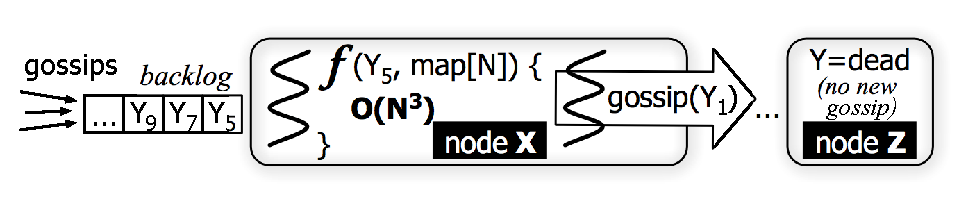
\includegraphics[height=0.8in]{F/cass1.eps}
%\includegraphics[height=0.6in]{F/empty.eps}
}
\vminfive
\mycaption[The problem of gossip-based failure detection in
Cassandra]{fig-cass1}{The problem of gossip-based failure detection in
Cassandra}{}
\vminfive
\end{figure}



To understand this bug, we need to understand the following protocols.
\begin{itemize}
\item {\bf Bootstrap:} Each node first creates partition keys (\eg, 32
random numbers) and gossips this information to peer nodes.
\item {\bf Gossip broadcast:} {\em Every second}, each node gossips to one 
random node about a list of nodes and partitions it knows (including
itself) and their {\em version} numbers.  Each node also increments its 
version number (``I'm still alive'') before gossiping.
\item {\bf Gossip processing:} The receiving node then finds any state
(metadata) differences between the two nodes to synchronize their views of
the ring.  Eventually, all nodes know about each other.
\item {\bf Failure detection:} {\em Every second}, a failure detection
daemon runs \cite{Lakshman+09-Cassandra}.  Put simply, if a node X has not 
received a new gossip about Y {\em from anyone} (Y's version has not 
changed after some period of time), X will declare Y dead (a flap).  When
X receives a new gossip about Y, it marks Y alive.
\end{itemize}

% about the bug
There are two factors that induce the bug.  The first is the {\em long latency
of scale-dependent state-update gossip processing during bootstrapping} (``f''
in Figure \ref{fig-cass1}).  While gossip processing is usually fast in a stable
cluster, it is expensive during bootstrapping as the gossips carry many new
state changes about the ring; the state-update processing time is
scale-dependent ($O(N^3)$); the larger the cluster ($N$), the larger the ring
map, the longer the processing time is.
%
This long latency is caused by {\bf (1)} state-update checkpoint to on-disk
database and {\bf (2)} multi-map cloning and updates.
%
The first one is needed for fast fault tolerance; after a node crashes, it can
reboot fast as it knows the latest view of the ring.
%
The second one is preferred for simplicity; Cassandra clones its \ts{MultiMap}
ring table and applies changes one by one to alleviate long write locks.
%
% in order to prevent a long write lock on the ring table which can block other
% user-facing protocols.

% long
The second factor is the {\em single threaded} implementation of gossip
processing.  As shown in Figure \ref{fig-cass1},  this inability to process
multiple gossips/state updates concurrently (for the sake of preventing
concurrency bugs) creates a {\em backlog} of new gossips.  For example, in {\em
every second}, Y tells someone it's alive with increasing version number (\eg,
Y$_7$), but the receiving nodes are still busy processing state changes and only
forward Y's old version number (\eg, Y$_1$).  As Y's new gossip is not
propagated on time,  other nodes (\eg, Z) will mark Y as dead.  This happens to
all nodes, not just Y.


\if 0
We mined bug repositories of four popular P2P key-value stores 
(Cassandra, Riak and 
Voldemort, Couchbase) and found \numStudy\footnote{The following are the 
  bugs we study (\textbf{with embedded hyperlinks}).
%
Cassandra: \caa, \cab, \cac, \cad, \cae ;
%
Couchbase: \cba, \cbb, \cbc, \cbd ;
%
Riak: \rka, \rkb ; and 
%
Voldemort: \vda.
%
This manual mining was arduous because there is no
standard jargon for ``scalability bugs'';
we might have missed other related bugs.
%
%For brevity, we only describe one bug in detail (\sec\ref{mot-bug})
%as the others have similar characteristics (\sec\ref{mot-observe}).
} control-plane scalability bugs.
%
These bugs caused significant availability problems such as long cluster
instability.
%
They also have complex characteristics (\sec\ref{mot-observe}).
\fi

\subsection{Observations}
\label{sec-scobs}

From the bug above, we make several important observations regarding
control-plane scalability bugs and distributed

\begin{itemize}
% only appear in large scale .. 
\item {\em Only appear at extreme scale:} \caone\ does not surface in 30-node
deployment. In 128-node cluster, the symptom appears mildly (tens of flaps).
From 200-500 nodes, flapping skyrockets to thousands of flaps. Testing in
small/medium scales is not sufficient.

% theory is not enough
\item {\em Scalable in design, but not in practice.}  Related to \caone, the
accrual failure detector \cite{Hayashibara+04-PhiFailureDetector} in
Cassandra is scalable in design \cite{Lakshman+09-Cassandra}.  However, the
design proof does not account gossip processing time, which can be long. To
understand the bug, the developers tried to ``do the [simple] math''
\cite{CA-One} but failed. In practice, new gossips are not propagated every
second (due to the backlog). The actual implementations overload gossips with
many other purposes (\eg, announcing boot/rebalance changes) beyond their
original design sketch.


% deep
\item {\em Implementation specific and hard to predict.}  The
backlog-induced flapping in \caone\ was caused specifically by Cassandra's
implementation choice: metadata checkpoint, multi-map cloning, and its
single-threaded implementation.  State-update processing time is hard to
predict (ranges from 0.001 to 4 seconds) as it depends on a 2-dimensional
input: the receiving node's ring table size and the number of new
state changes (\sec\ref{sec-eval}).

% not independent
\item {\em Cascading impacts of ``not-so-independent'' nodes.}  In
cluster-wide control protocols, distributed nodes are  not
necessarily independent; nodes must communicate with each other
to synchronize their views of cluster metadata.  As the cluster grows, the
cluster metadata size increases.  Thus, unpredictable processing time in
individual nodes can create cascading impacts to the whole cluster.

% 
\item {\em Long and difficult large-scale debugging:}
%
The bug report of \caone\ generated over 40 back-and-forth discussion
comments and took 2 months to fix.  It is apparent \cite{CA-One} that
there were many hurdles of deploying and debugging the buggy protocol at
real scale.  Important to note is that debugging is {\em not} a single
iteration; developers must {\em repeatedly} instrument the system (add
more logs) and re-run the system at scale to find and fix the bug, which
is not trivial.  The scalability bugs we studied took 6 to 157 days to
fix (27 on average).

\item {\em Not all developers have large test budgets:}
%
Another factor of delayed fixes is the lack of budget for large
test clusters.  Such luxury tends to be accessible to developers
in large companies, but not to
open-source developers.  When
\caone\ was submitted by a customer who had hundreds of nodes, the
Cassandra developers did not have an instant access to a test cluster of
the same scale.

% repeated 
\item {\em Quick fixes and repeated bugs:} Bugs are often fixed with quick
patches (development pressures), but the fix might not eradicate the problem
completely \cite{Yin+11-FixesBecomeBugs}.
%
The patch for \caone\ simply disables failure detection during bootstrap. But
the bug still appeared in another workload (\eg, scaling out from 128 to 256
nodes).
%
The simple fix has been removed later and the gossip protocol has been
redesigned.
%
And old fixes can become obsolete in protocol re-designs, which then can give
birth to new scalability bugs such as the fix for \csb{3831} became obsolete as
``vnodes'' was introduced, then led to a new scalability bug (\csb{3881}).

\end{itemize}

\subsection{State of the Art}

We now discuss popular approaches (simulation, extrapolation, and emulation) for
unearthing scalability bugs.
% ......
First, simulation approaches test system/application models in different scales
\cite{Calotoiu+13-ApmScaleBug, Laguna+15-DebugAtScale}. A model can look
scalable but the actual implementation can contain unforeseen bugs. Our
observations above accentuate the need for scale-checking distributed system
{\em implementations} at {\em real scale}.


% --------------- mini cluster
Second, extrapolation monitors system behaviors in ``mini clusters'' and 
extrapolates them to larger scales (\sec2.1 in \cite{Wang+14-Exalt}).
However, mini clusters tend to be order(s) of magnitude smaller than real
deployments.
% (\sec2.2 in \cite{Leesatapornwongsa+14-Drill}).  
% Not all
% developers have the luxury of mini clusters (\eg, ``mini'' can imply
% hundreds nodes in large companies).  
Most importantly, system behaviors do not always extrapolate linearly
\cite{Wang+14-Exalt}; for the bugs in our work (\sec\ref{sec-eval}), even an
extrapolation based on a 100-node cluster will not reveal the bug symptoms.

% --------------- emulation
Finally, real-scale emulation checks real implementations in an emulated
environment (\eg, DieCast and Exalt).
%
DieCast \cite{Gupta+08-DieCast}, invented for network emulation, can 
colocate many processes/VMs on a single machine as if they run 
individually without contention.  The trick is adding ``time dilation
factor'' (TDF) support \cite{Gupta+06-TimeDilation} into the VMM (\eg, Xen).
%
For example, TDF=5 implies that for every second of wall-clock time, each
emulated VM on the VMM believes that time has advanced by only 200 ms. 
%
The most significant drawback of DieCast is that high colocation factor
(\eg, TDF$=$100) is likely not desirable, for two reasons: prolonged
testing time (TDF$=$100 implies 100x longer run) and memory overcapacity.
%
Many distributed systems today are implemented in managed languages (\eg, Java,
Erlang) whose runtimes consume non-negligible memory overhead. Java and Erlang
VMs for example use around 70 and 64 MB of memory per process respectively. 
%
DieCast was only evaluated with TDF=10.

% co-location -- data compression -- exalt
Exalt \cite{Wang+14-Exalt} targets I/O-intensive scalability bugs.  With a
custom data compression, users' data is compressed to zero byte on disk (but the
size is recorded) while metadata is not compressed.  With this, Exalt can
co-locate 100 emulated HDFS datanodes on one machine.  In its evaluation, most
of the bugs reproduced are in the HDFS namenode which runs alone on one machine.
As the authors stated, their approach ``may not discover scalability problems
that arise at the nodes that are being emulated [the datanodes]'' (\sec4.1 in
\cite{Wang+14-Exalt}).  Thus, Exalt is not suitable for finding control-plane
scalability bugs in P2P distributed systems.

% P2P systems \cite{sosp01-past}.

% for control-plane
In summary, we did not find a fast single-machine approach that can scale-check
control-plane protocols in P2P systems.
%
The scalability bugs here are typically caused by the scale-dependent processing
time, not network or I/O bottlenecks.  As DieCast targets {\em network}
emulation via time dilation and Exalt targets {\em storage} space emulation via
compression, our work uniquely targets {\em processing time} emulation,
completing a missing piece.


\section{Conclusion}

In this chapter, we discuss about cloud-scale distributed systems, software
backend for the cloud computing. We show what the current trend of the systems
is and how they are design. We also discuss about distributed concurrency and
scalability, the two important aspects of cloud-scale distributed systems that
could threaten dependability of the systems. We briefly discuss how system
community address issues from the concurrency and scalability. Unfortunately,
distributed concurrency bugs are still an unsolved problem, and scalability bugs
are novel and not many works address about them.



\input{main-detail}
\chapter{Research Plan}
\label{chp-plan}

To unearth bugs in cloud-scale distributed systems, the first thing we need is
comprehensive knowledge about them, so we can establish proper solutions. In our
research plan, we start with general bug study on cloud systems to see the big
picture of the current problems. Then we dissect DC bugs and scalability bugs to
analyze.
%
For DC bugs, we will advance the state of the art of dmcks. We are introducing 
more pruning policies to tackle state-space explosion problem. And for
scalability bugs, we will fill the missing piece of control-plane protocol bugs
focusing on P2P systems.

\section{Bug Study}

Bug or failure studies can significantly guide many aspects of dependability
research. Many dependability researchers have recently employed formal studies
on bugs and failures such as the studies on large-scale system bugs/failures
from Microsoft \cite{Guo+13-CureIsWorse, Li+13-ScopeBugStudy} These studies can
identify opportunities for new research, build taxonomies of new problems, or
test new tools. I started my research by doing formal bug study to gain
foundations of combating DC bugs.

\subsection{Cloud Bug Study}

As an initiative, our group have performed the largest bugs study in six 
important Apache cloud infrastructures including Cassandra, Flume, Hadoop
MapReduce, HBase, HDFS, and ZooKeeper \cite{Gunawi+14-Cbs}. We reviewed in
total 21,399 submitted issues within a three-year period (2011-2014) in Apache
bug repositories. We perform a deep analysis of 3,655 ``vital'' issues (\ie,
real issues affecting deployments) with a set of detailed classifications. This
work led us to several interesting dependability research questions, and was 
the main source of my DC-bug taxonomy work.

\subsection{DC Bug Taxonomy} 

While there have been many LC-bug studies, I am not aware of any large-scale
study of DC bugs. A recent study from Microsoft analyzed the effect of
distributed concurrency on workload and only studied five DC bugs in MapReduce
systems \footnote{Tian Xiao, Jiaxing Zhang, Hucheng Zhou, Zhenyu Guo, Sean
McDirmid, Wei Lin, Wenguang Chen, and Lidong Zhou. Nondeterminism in MapReduce
Considered Harmful?  An Empirical Study on Non-commutative Aggregators in
MapReduce Programs. ICSE '14}. To fill the void, I as one of the project
leaders, have created the largest and most comprehensive taxonomy of 104
real-world DC bugs (named \taxdc) from Cassandra, HBase, Hadoop MapReduce/Yarn,
and ZooKeeper \cite{Leesatapornwongsa+16-TaxDc}. \taxdc\ contains in-depth
characteristics of DC bugs, stored in the form of 2,083 classification labels
and 4,528 lines of re-enumerated steps to the bugs that I manually added.
Motivated by the availability of bug benchmarks for LC bugs, I will release
\taxdc\ as a large-scale DC bugs benchmark.

With \taxdc\, I can answer important questions such as: How often are DC bugs
reported from real deployments? What types of DC bugs exist in real world?
What are the root causes of DC bugs (out-of-order messages, failures, \etc)?
Are existing LC-bug-detection tools applicable for DC bugs? How do developers
fix DC bugs (by adding locks, states, \etc)? What are the inputs/triggering
conditions?  What are the minimum number of distributed events needed to
trigger the bugs (how many messages to re-order, failures to inject, \etc)?
What errors/effects (specification violations) are caused by DC bugs (deadlock,
data loss, state inconsistency, performance problems, \etc)? How do propagation
chains form from the root causes to errors? The answers to these questions will
guide my subsequent research projects.

\section{Distributed System Model Checking}

One powerful method for discovering hidden DC bugs is the use of an
\textit{implementation-level distributed system model checker} (\textbf{dmck}).
By re-ordering non-deterministic distributed events, a dmck can discover buggy
interleavings that lead to DC bugs. The last eight years have seen a rise of
dmcks such as MaceMC \footnote{Charles Killian, James Anderson, Ranjit Jhala,
and Amin Vahdat. Life, Death, and the Critical Transition: Finding Liveness Bugs
in Systems Code. NSDI '07}, \modist\ \cite{Yang+09-Modist}, or Demeter 
\cite{Guo+11-Demeter}. One big challenge faced by a dmck is the
state-space explosion problem (\ie, there are too many distributed events to
re-order). To address this, existing dmcks adopt a random walk or basic
reduction techniques such as dynamic partial order reduction (DPOR). Despite
these early successes, existing approaches cannot unearth many real-world DC
bugs, so I am advancing the state of the art of dmck to combat DC bugs, which I
describe below.

\subsection{Semantic-Aware Model Checking (Initial Work)}

I started my work by specifically addressing two limitations of existing dmcks.
First, existing dmcks treat every target system as a complete \textit{black
box}, and therefore perform unnecessary reorderings of distributed events that
would lead to the same explored states (\ie, redundant executions). Second,
they do not incorporate complex multiple fault events (\eg, crashes, reboots)
into their exploration strategies, as such inclusion would exacerbate the
state-space explosion problem.

To address these limitations, I built Semantic-Aware Model Checking
(\textbf{SAMC}) \cite{Leesatapornwongsa+15-SamcIssta,Leesatapornwongsa+14-Samc},
a novel white-box model checking approach that takes \textit{semantic knowledge}
of how distributed events (specifically, messages, crashes, and reboots) are
processed by the target system and incorporates that information in reduction
policies.  The policies are based on sound reduction techniques such as DPOR and
symmetry.  The policies tell SAMC not to re-order some pairs of events such as
message-message pairs or crash-message pairs, yet preserves soundness, because
those cut out re-orderings are redundant.

I built SAMC from scratch with 10 KLOC and I was able to reproduce 12 old bugs
in 3 cloud systems involving 30-120 distributed events and multiple crashes and
reboots. Some of these bugs cannot be unearthed by non-SAMC approaches, even
after two days. SAMC can find the bugs up to 271x (33x on average) faster
compared to state-of-the-art techniques. Additionally, I found two new bugs in
Hadoop MapReduce and ZooKeeper.



\section{Distributed System Model Checking}

One powerful method for discovering hidden DC bugs is the use of an
\textit{implementation-level distributed system model checker} (\textbf{dmck}).
By re-ordering non-deterministic distributed events, a dmck can discover buggy
interleavings that lead to DC bugs. The last eight years have seen a rise of
dmcks such as MaceMC \cite{Killian+07-LifeDeathMaceMC} 
\modist\ \cite{Yang+09-Modist}, or Demeter 
\cite{Guo+11-Demeter}. One big challenge faced by a dmck is the
state-space explosion problem (\ie, there are too many distributed events to
re-order). To address this, existing dmcks adopt a random walk or basic
reduction techniques such as dynamic partial order reduction (DPOR). Despite
these early successes, existing approaches cannot unearth many real-world DC
bugs, so I am advancing the state of the art of dmck to combat DC bugs, which I
describe below.

\subsection{Semantic-Aware Model Checking}

I started my work by specifically addressing two limitations of existing dmcks.
First, existing dmcks treat every target system as a complete \textit{black
box}, and therefore perform unnecessary reorderings of distributed events that
would lead to the same explored states (\ie, redundant executions). Second,
they do not incorporate complex multiple fault events (\eg, crashes, reboots)
into their exploration strategies, as such inclusion would exacerbate the
state-space explosion problem.

To address these limitations, I built Semantic-Aware Model Checking
(\textbf{SAMC}) \cite{Leesatapornwongsa+15-SamcIssta,Leesatapornwongsa+14-Samc},
a novel white-box model checking approach that takes \textit{semantic knowledge}
of how distributed events (specifically, messages, crashes, and reboots) are
processed by the target system and incorporates that information in reduction
policies.  The policies are based on sound reduction techniques such as DPOR and
symmetry.  The policies tell SAMC not to re-order some pairs of events such as
message-message pairs or crash-message pairs, yet preserves soundness, because
those cut out re-orderings are redundant.

I built SAMC from scratch with 10 KLOC and I was able to reproduce 12 old bugs
in 3 cloud systems involving 30-120 distributed events and multiple crashes and
reboots. Some of these bugs cannot be unearthed by non-SAMC approaches, even
after two days. SAMC can find the bugs up to 271x (33x on average) faster
compared to state-of-the-art techniques. Additionally, I found two new bugs in
Hadoop MapReduce and ZooKeeper.




\input{plan-sck}


\chapter{Summary}
\label{chp-con}

In this proposal, we aim to unearth hidden bugs in cloud-scale distributed
systems that weaken reliability and scalability of the systems. For reliability
bugs, we focus in distributed concurrency (DC) bugs. For scalability bugs, we
focus in control-plane protocol bug, specifically in P2P storage systems.

The key idea for unearthing DC bugs is advancing model checking techniques. 



% Format a LaTeX bibliography
\makebibliography

% Figures and tables, if you decide to leave them to the end
%\input{figure}
%\input{table}

\end{document}


